\subsection{Dataset in lingua inglese} \label{ner_eng_data}
\label{sec:ner_dataset_en}
Il dataset utilizzato è la versione in inglese del task CoNLL-2003, disponibile nella repository Github\footnote{Dataset: \href{https://github.com/JohnSnowLabs/spark-nlp/tree/master/src/test/resources/conll2003}{https://github.com/JohnSnowLabs/spark-nlp/tree/master/src/test/resources/conll2003}} di Spark NLP. 

Il dataset è composto da tre file: \textit{eng.train} con 14.041 esempi per l’addestramento, \textit{eng.test} con 6.603 esempi per il testing.

Il primo elemento su ogni riga è una parola, il secondo un tag \textbf{part-of-speech (POS)}, il terzo un tag \textbf{chunk sintattico} e il quarto il tag \textbf{named entity}. I tag chunk e i tag named entity hanno il formato \textit{I-TYPE} che significa che la parola è dentro una frase di tipo \textit{TYPE}. Solo se due frasi dello stesso tipo si susseguono immediatamente, la prima parola della seconda frase avrà il tag \textit{B-TYPE} per mostrare che inizia una nuova frase. Una parola con il tag \textit{O} non fa parte di una frase. Le entità presenti nel dataset sono: \textit{persone}, \textit{luoghi}, \textit{organizzazioni} ed entità \textit{varie} che non appartengono ai tre gruppi precedenti.
\begin{figure}[hbt!]
    \centering
    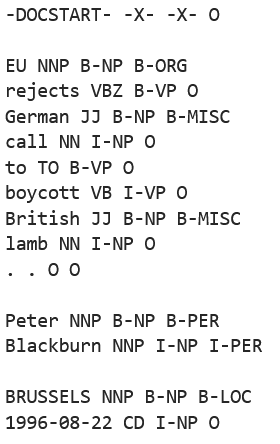
\includegraphics[width=0.25\textwidth]{img/ner_en_dataset.png}
    \caption{Porzione del dataset per NER in lingua inglese}
    \label{fig:ner_en_dataset}
\end{figure}
